\section{Results}
\subsection{Parameters}

\begin{figure*}
\centering

\subfigure
{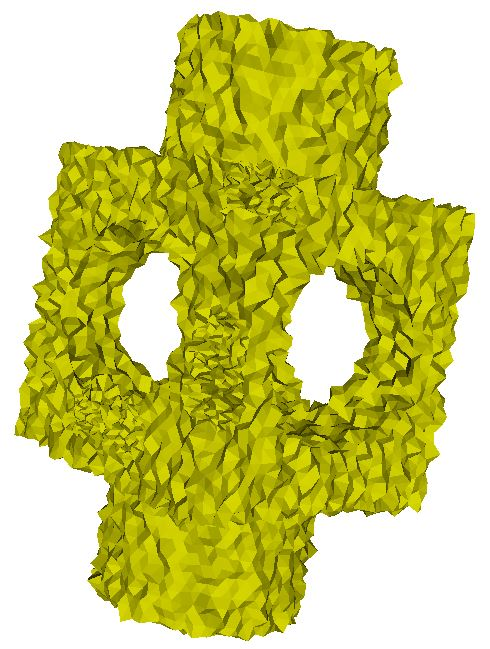
\includegraphics[width = 1.8cm]{results/block_Noisy.jpg}}
\subfigure
{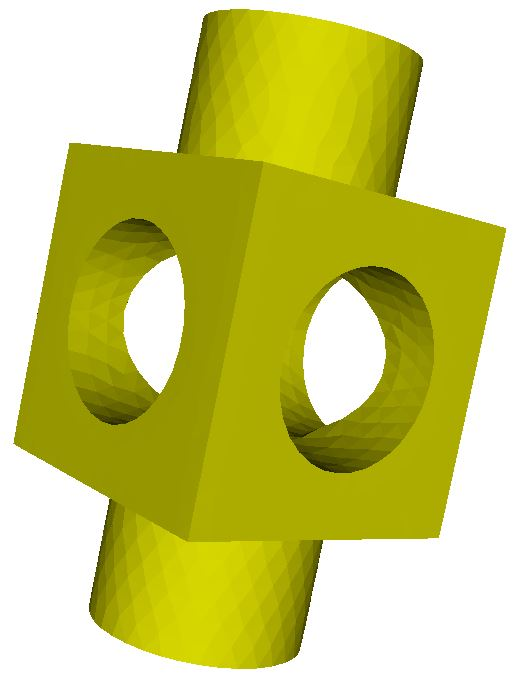
\includegraphics[width = 1.8cm]{results/block_Original.jpg}}
\subfigure
{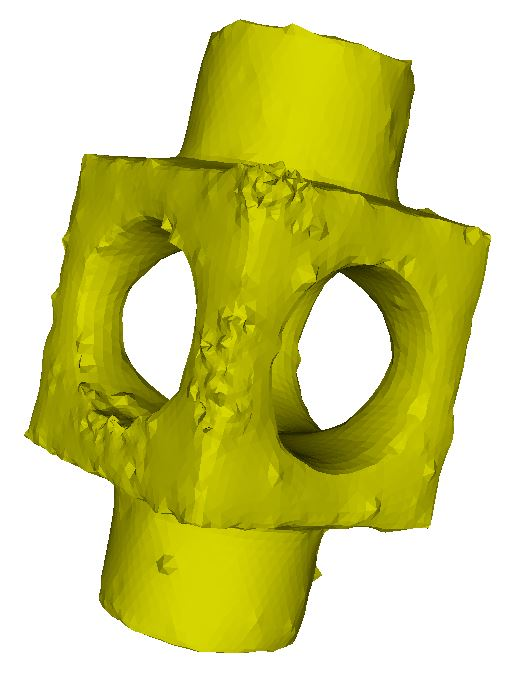
\includegraphics[width = 1.8cm]{results/block_FDCO03.jpg}}
\subfigure
{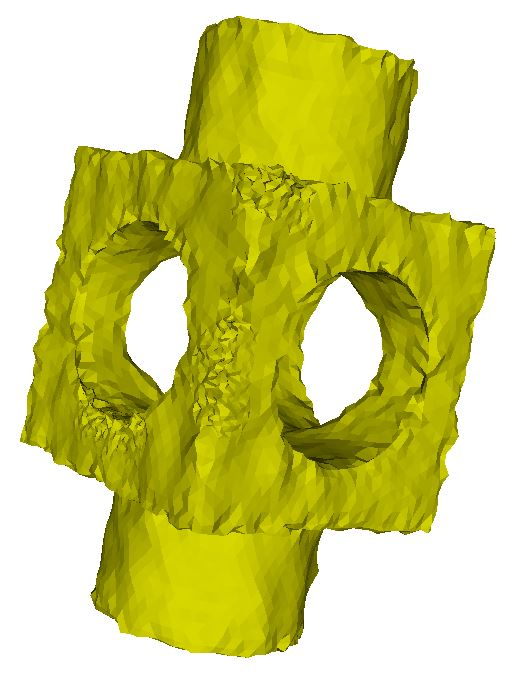
\includegraphics[width = 1.8cm]{results/block_JDD03.jpg}}
\subfigure
{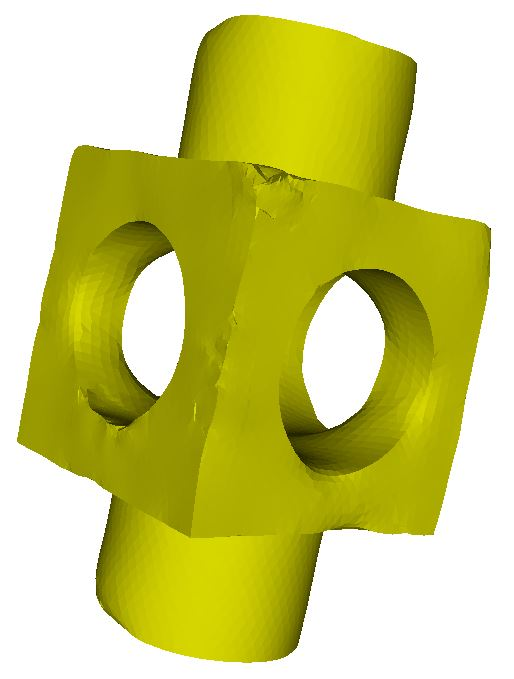
\includegraphics[width = 1.8cm]{results/block_SRML07.jpg}}
\subfigure
{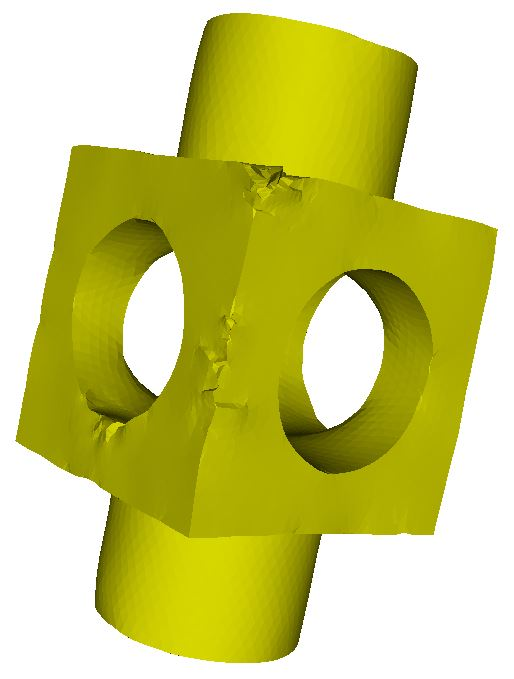
\includegraphics[width = 1.8cm]{results/block_ZFAT11local.jpg}}
\subfigure
{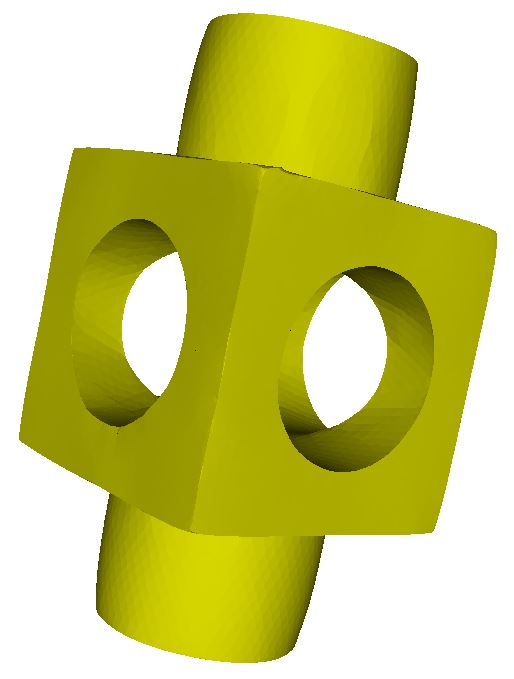
\includegraphics[width = 1.8cm]{results/block_HS13.jpg}}
\subfigure
{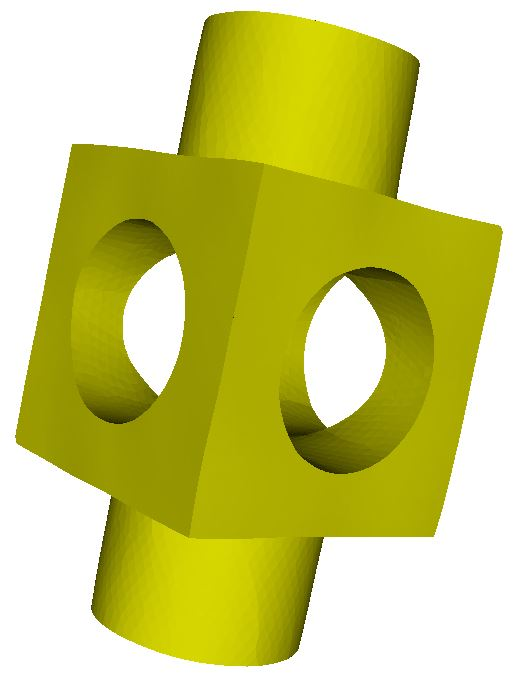
\includegraphics[width = 1.8cm]{results/block_PG15.jpg}}
\subfigure
{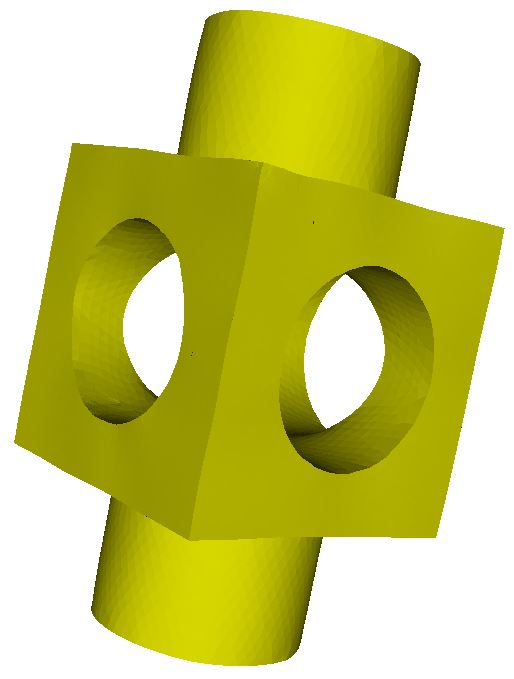
\includegraphics[width = 1.8cm]{results/block_our.jpg}}
\\
\vspace{-1.2mm}

\subfigure
{\includegraphics[width = 1.8cm]{results/twelve_Noisy.jpg}}
\subfigure
{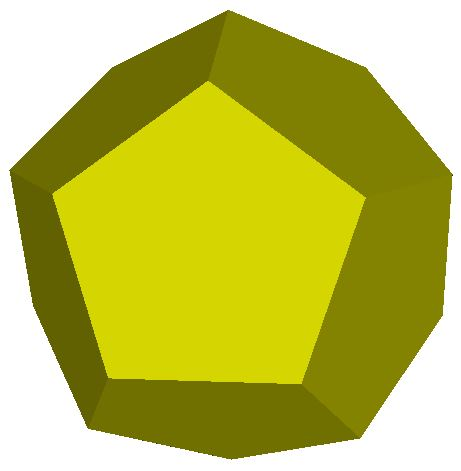
\includegraphics[width = 1.8cm]{results/twelve_Original.jpg}}
\subfigure
{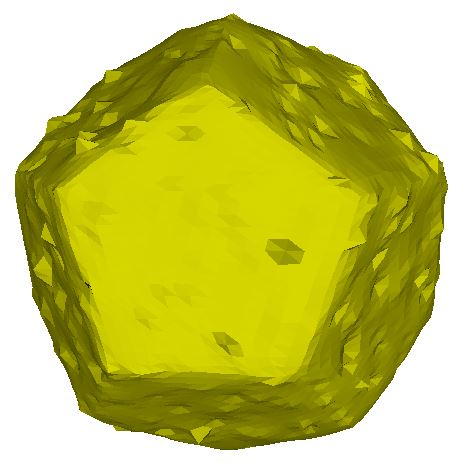
\includegraphics[width = 1.8cm]{results/twelve_FDCO03.jpg}}
\subfigure
{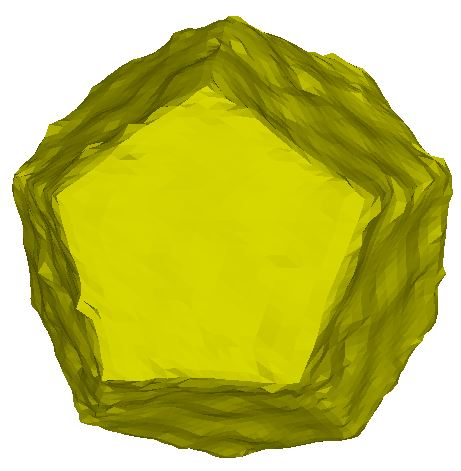
\includegraphics[width = 1.8cm]{results/twelve_JDD03.jpg}}
\subfigure
{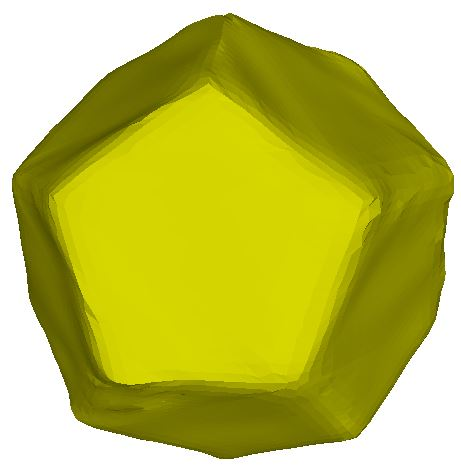
\includegraphics[width = 1.8cm]{results/twelve_SRML07.jpg}}
\subfigure
{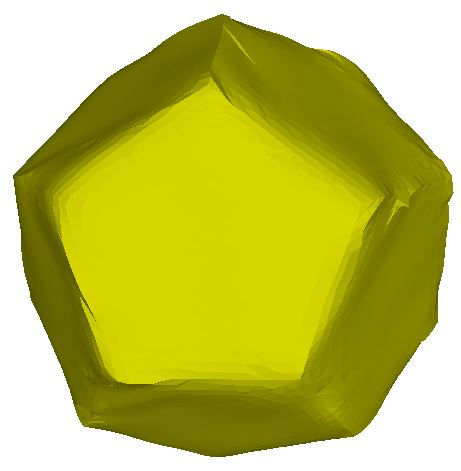
\includegraphics[width = 1.8cm]{results/twelve_ZFAT11local.jpg}}
\subfigure
{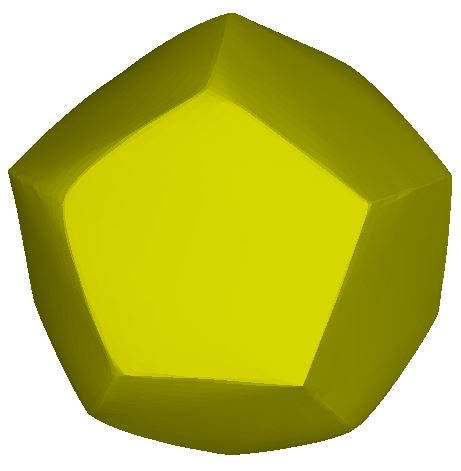
\includegraphics[width = 1.8cm]{results/twelve_HS13.jpg}}
\subfigure
{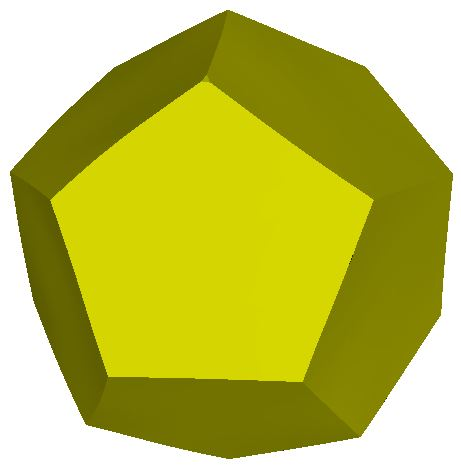
\includegraphics[width = 1.8cm]{results/twelve_PG15.jpg}}
\subfigure
{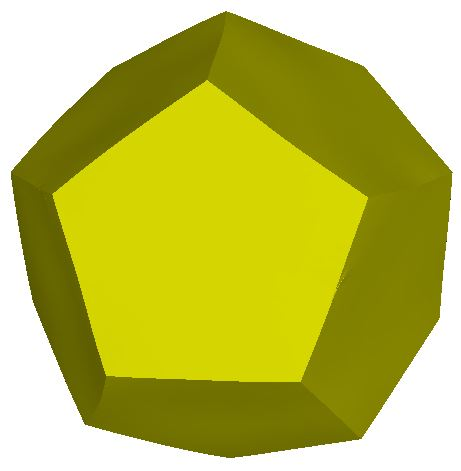
\includegraphics[width = 1.8cm]{results/twelve_our.jpg}}
\caption{ Comparisons with other methods on synthetic meshes.}
\label{Fig:special}
\end{figure*}

%\begin{figure*}
%\centering
%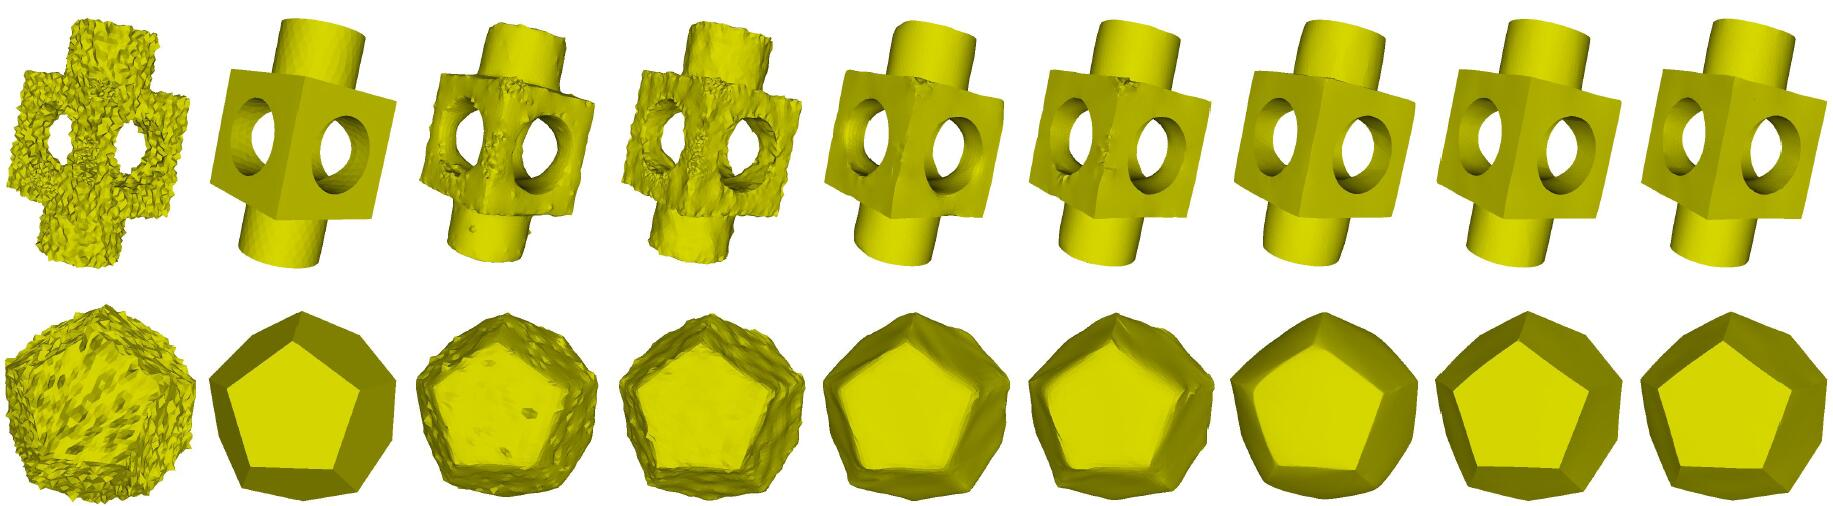
\includegraphics[width = 17.0cm]{results/irregularMesh.jpg}
%\vspace{0.5mm}
%\caption{ Denoising results using different values of $\sigma_r$ with other parameters fixed.}
%\label{Fig:sigma}
%\end{figure*}

Our method has four parameters: the number of normal filtering iterations $k_{iter}$,
the number of iterations $v_{iter}$ for vertex update,
choosing a radius parameter $r$ determined the geometrical neighborhood,
and the standard variance parameters $\sigma_s$ and $\sigma_r$, for the two difference between normals, respectively.
In our experiments, we find that $k_{iter}\leq80$ and $v_{iter}\leq5$ are enough for achieving satisfactory results.
For all results in this paper, we set the same value to $\sigma_s$ and $\sigma_r$ for employing the filtering unless stated otherwise.
And when their values are between 0.2 and 0.8, a good experimental result can be achieved.
Later, we will introduce the function of the standard variance parameters.
In addition, we choose $r\in[2d, 6d]$ where $d$ is the average distance between neighboring face centroids across the whole mesh.

\subsection{Results and comparisons}

In the following, we compare our denoising results with other methods on synthetic noisy meshes and real meshes.
And furthermore, for synthetic meshes, we also evaluate two quantitative metrics about vertex-based and normal-based mesh-to-mesh error metric
separately introduced in papers~\cite{belyaev2003comparison} and~\cite{nehorai2000performance} to analyze the difference between our results and others.

The vertex-based error metric is
\begin{equation}
\begin{aligned}
\label{Eq:vertexerror}
E_v = \sqrt{\frac{1}{3 A(M^{'})}\sum_{P^{'} \in M^{'}} A(P^{'}) dist(P^{'}, M)^2}\, ,
%E_v = \sqrt{\frac{1}{3A(M^')} \sum_{P^' \in M^'} A(P^') dist(P^', M)^2}\, ,
\end{aligned}
\end{equation}
where $M$ and $M^{'}$ reference original noiseless mesh and denoised mesh respectively, $P^{'}$ is a vertex of $M^{'}$
and $dist(P^{'}, M)$ defines the distance between $P^{'}$ and a triangle of $M$ which is closest to $P^{'}$.

The normal-based error metric is used to reveal the average angle offset which is defined as follows
\begin{equation}
\begin{aligned}
\label{Eq:vertexerror}
E_n = \sum_{f^{'} \in M^{'}, f \in M} angle(\mathbf{n^{'}}, \mathbf{n}) / N\, ,
%E_v = \sqrt{\frac{1}{3A(M^')} \sum_{P^' \in M^'} A(P^') dist(P^', M)^2}\, ,
\end{aligned}
\end{equation}
where $f^{'}$ and $f$ are triangle faces of $M^{'}$ and $M$ respectively,
$\mathbf{n^{'}}$ and $\mathbf{n}$ reference the normal of $f^{'}$ and $f$,
$angle(\mathbf{n^{'}}, \mathbf{n})$ defines the angle between $\mathbf{n^{'}}$ and $\mathbf{n}$
and the last $N$ is the number of triangle faces of a mesh.

We generate the synthetic meshes though adding Gaussian noise to the vertices of a ground truth mesh along the vertex normals.
The intensity of the noise is defined by a relative standard deviation $\sigma_E = \sigma / E_{mean}$,
where $\sigma$ is the standard deviation of the Gaussian function and $E_{mean}$ is the average edge length of the ground truth mesh.

From the results of figure~\ref{Fig:oct}, the approaches of Fleishman et al~\cite{fleishman2003bilateral} and Jones et al~\cite{jones2003non}
can not well preserve the strong edges, because the spatial weight weaken the strength of filtering.
While the rest of methods have the ability to maitain the mesh edge structure, they can not well deal with the sharp corner.
The main reason is that the methods of Sun et al~\cite{sun2007fast} and Zheng et al~\cite{zheng2011bilateral}(l) easily smooth the sharp corner,
The approaches of He et al~\cite{he2013mesh} and Zhang et al~\cite{Zhang2015Filter} are prone to ambiguity.
Because our method divide the neighborsets, it can well preserve the sharp cvorner and edge.


Figure~\ref{Fig:weakEdge} shows the efectiveness of our method on preserving weak edges.
The noisy model is a prism with 18 edges, the struct is not obvious.
We apply Gaussian noise to this model with the intensity $\sigma_E = 0.1$.
Other methods can not well restore these weak edges and easily smooth them.

In the figure~\ref{Fig:special} with two models selected from~\cite{Zhang2015Filter}, we show our method also can deal with different kinds of noise.
The types of noise are from top to down Gaussian noise with irregular sampling and impulsive noise separately.
And noisy intensity $\sigma_E$ are 0.4 and 0.5 separatly.
From the vision,  our method almost obtain the similar results comparing with Zhang et al~\cite{Zhang2015Filter}.
However, according to the table\ref{tab:1}, our method obtains better results.

\begin{figure*}
\centering

\subfigure
{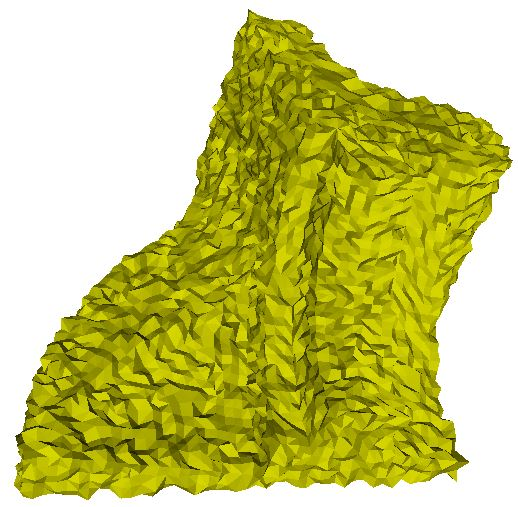
\includegraphics[width = 1.8cm]{results/fandisk_Noisy.jpg}}
\subfigure
{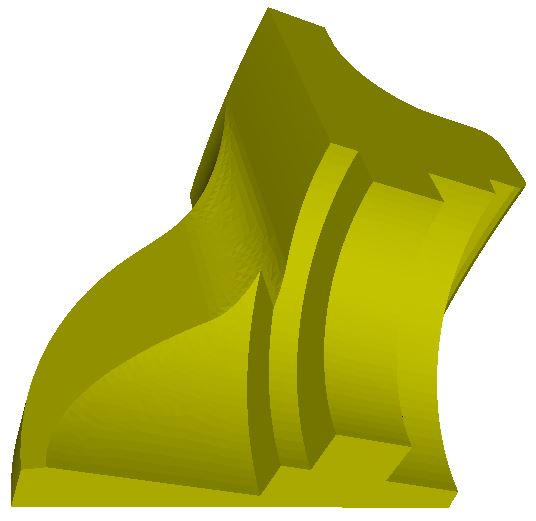
\includegraphics[width = 1.8cm]{results/fandisk_Original.jpg}}
\subfigure
{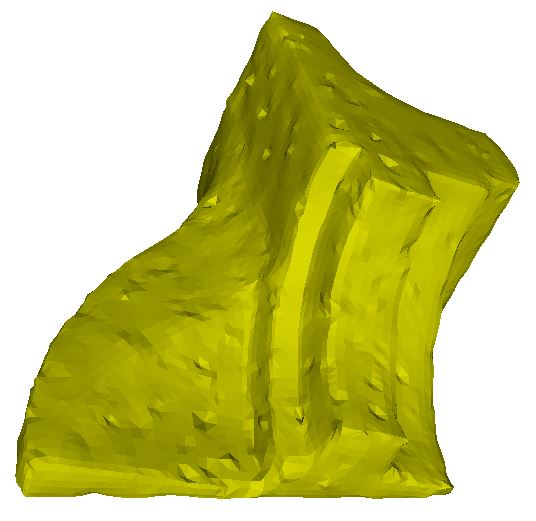
\includegraphics[width = 1.8cm]{results/fandisk_FDCO03.jpg}}
\subfigure
{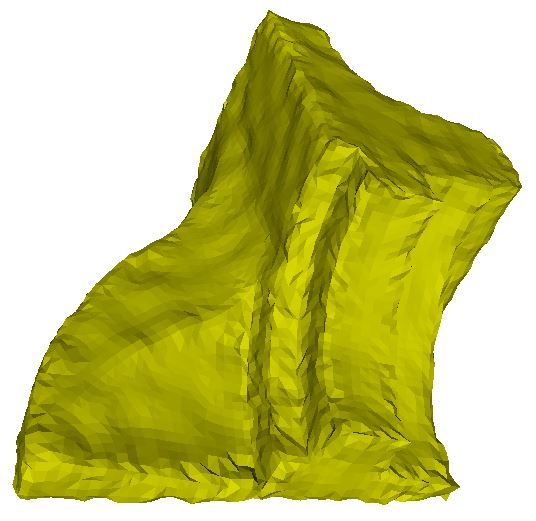
\includegraphics[width = 1.8cm]{results/fandisk_JDD03.jpg}}
\subfigure
{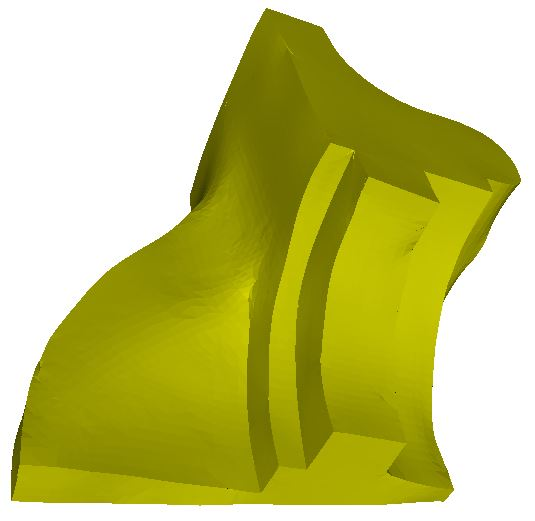
\includegraphics[width = 1.8cm]{results/fandisk_SRML07.jpg}}
\subfigure
{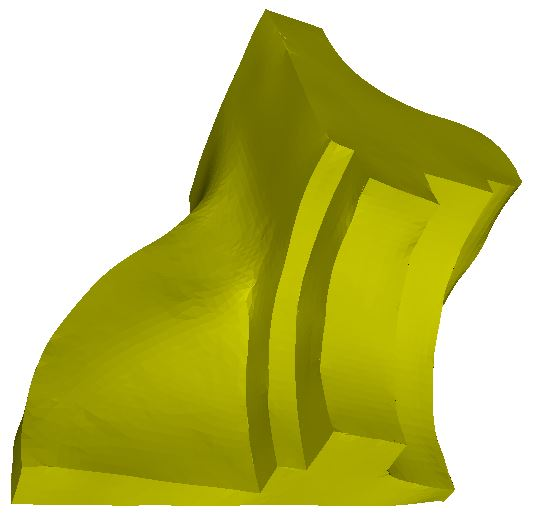
\includegraphics[width = 1.8cm]{results/fandisk_ZFAT11local.jpg}}
\subfigure
{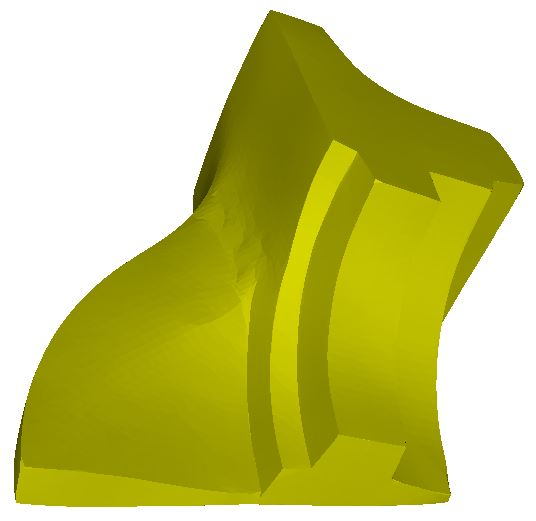
\includegraphics[width = 1.8cm]{results/fandisk_HS13.jpg}}
\subfigure
{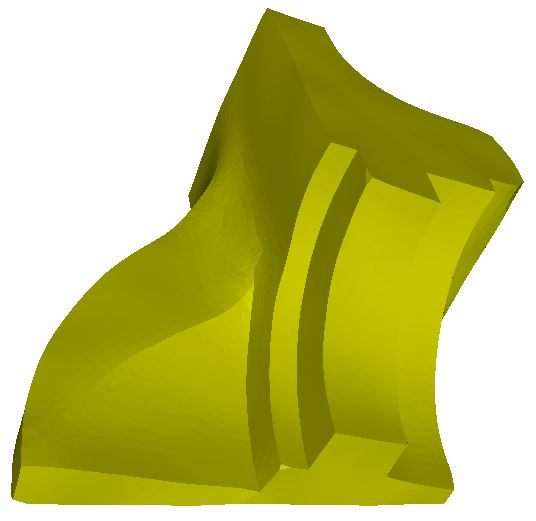
\includegraphics[width = 1.8cm]{results/fandisk_PG15.jpg}}
\subfigure
{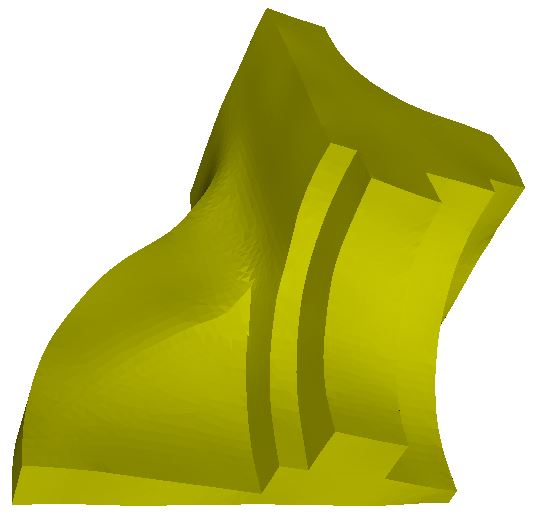
\includegraphics[width = 1.8cm]{results/fandisk_our.jpg}}
\\
\vspace{-1.2mm}

\subfigure
{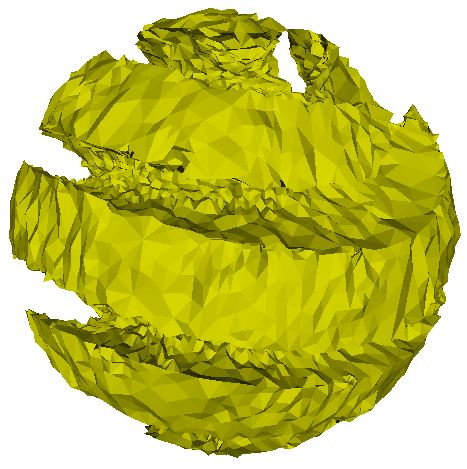
\includegraphics[width = 1.8cm]{results/sphere_Noisy.jpg}}
\subfigure
{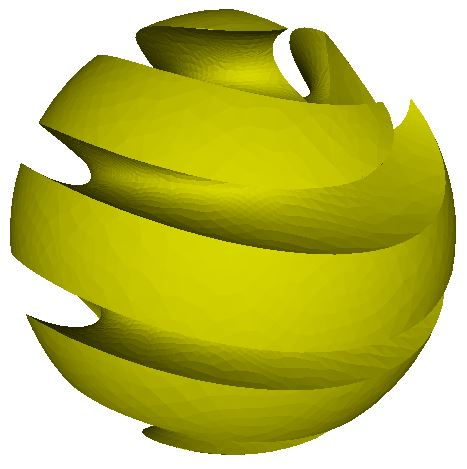
\includegraphics[width = 1.8cm]{results/sphere_Original.jpg}}
\subfigure
{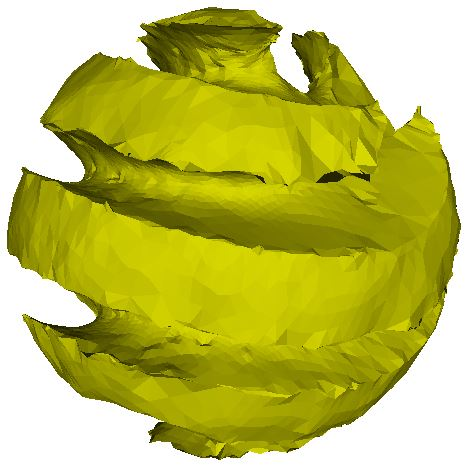
\includegraphics[width = 1.8cm]{results/sphere_FDCO03.jpg}}
\subfigure
{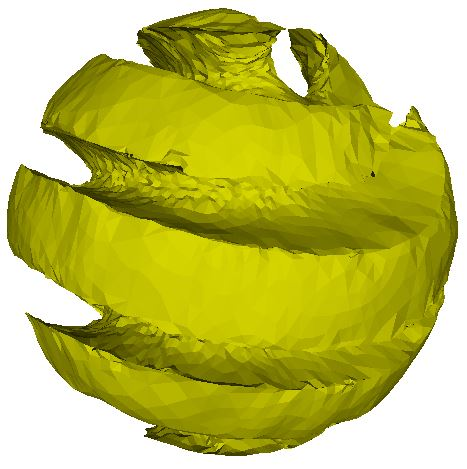
\includegraphics[width = 1.8cm]{results/sphere_JDD03.jpg}}
\subfigure
{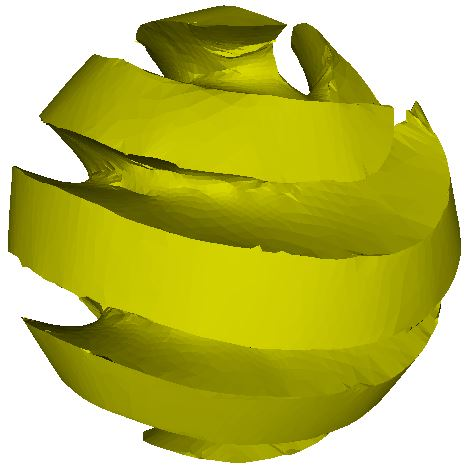
\includegraphics[width = 1.8cm]{results/sphere_SRML07.jpg}}
\subfigure
{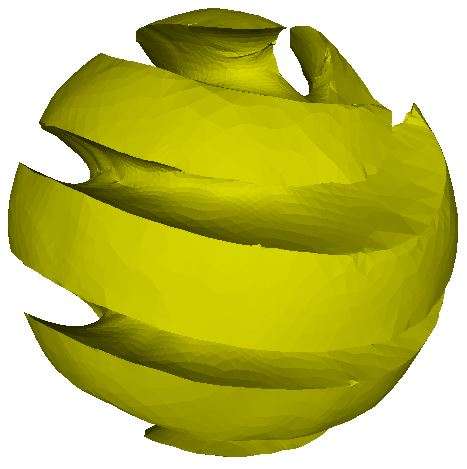
\includegraphics[width = 1.8cm]{results/sphere_ZFAT11local.jpg}}
\subfigure
{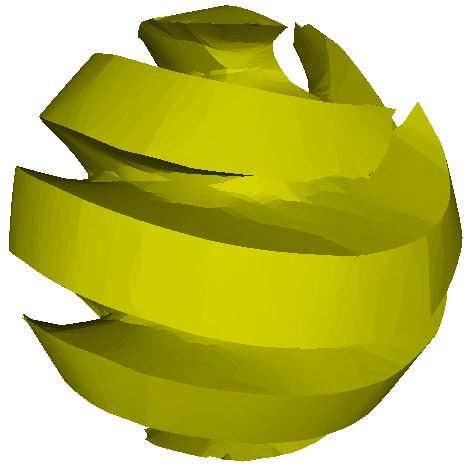
\includegraphics[width = 1.8cm]{results/sphere_HS13.jpg}}
\subfigure
{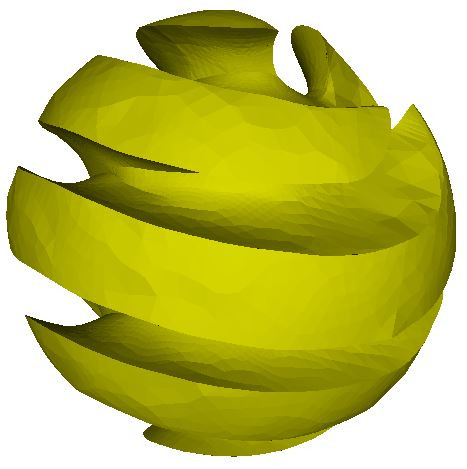
\includegraphics[width = 1.8cm]{results/sphere_PG15.jpg}}
\subfigure
{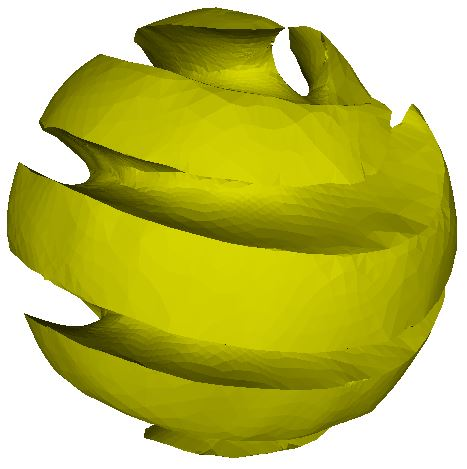
\includegraphics[width = 1.8cm]{results/sphere_our.jpg}}
\\
\vspace{-1.2mm}

\subfigure
{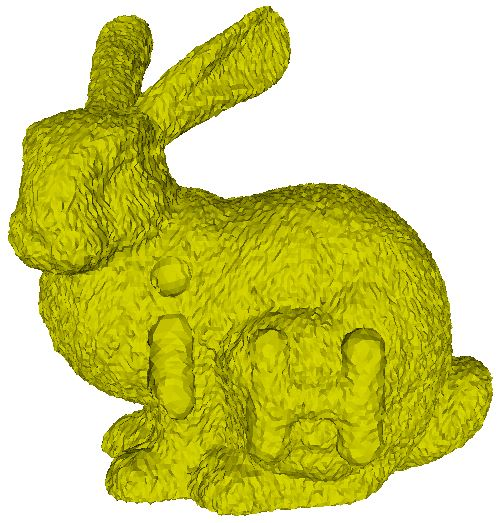
\includegraphics[width = 1.8cm]{results/bunny_Noisy.jpg}}
\subfigure
{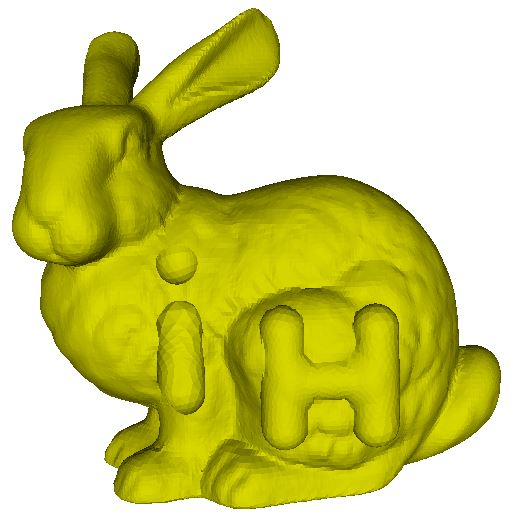
\includegraphics[width = 1.8cm]{results/bunny_Original.jpg}}
\subfigure
{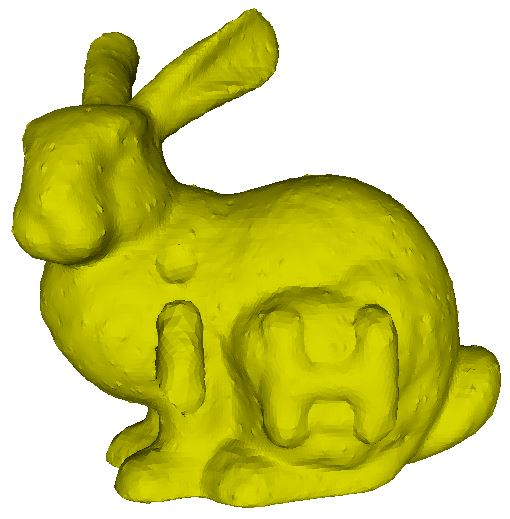
\includegraphics[width = 1.8cm]{results/bunny_FDCO03.jpg}}
\subfigure
{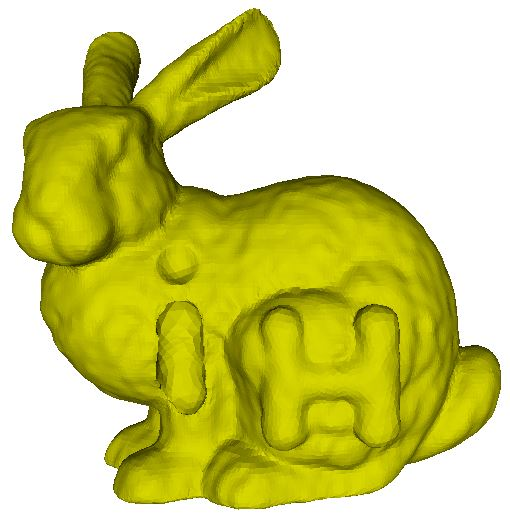
\includegraphics[width = 1.8cm]{results/bunny_JDD03.jpg}}
\subfigure
{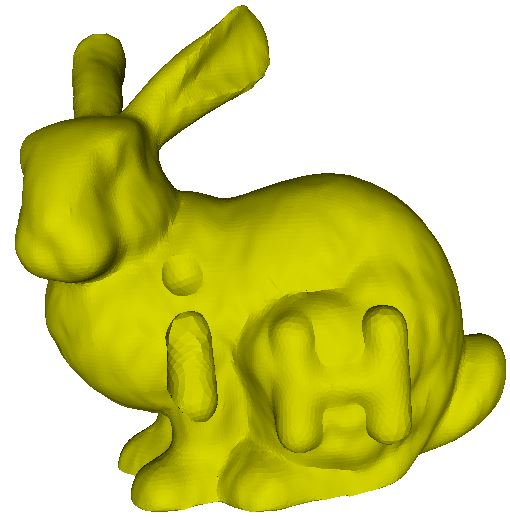
\includegraphics[width = 1.8cm]{results/bunny_SRML07.jpg}}
\subfigure
{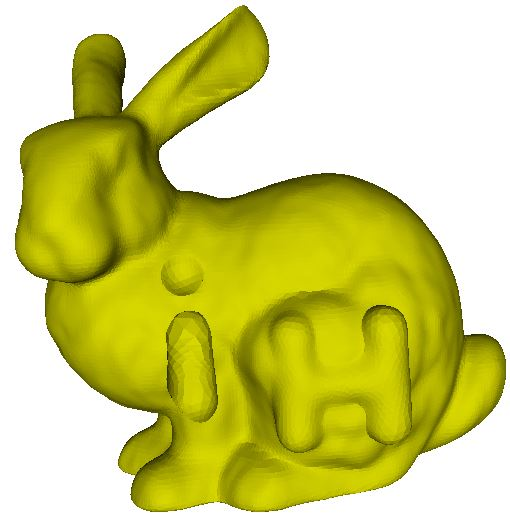
\includegraphics[width = 1.8cm]{results/bunny_ZFAT11local.jpg}}
\subfigure
{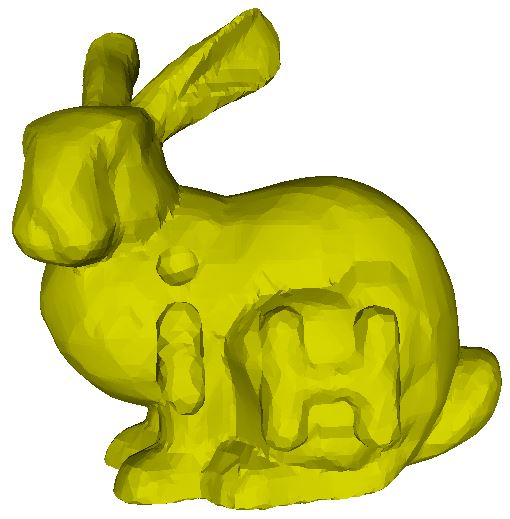
\includegraphics[width = 1.8cm]{results/bunny_HS13.jpg}}
\subfigure
{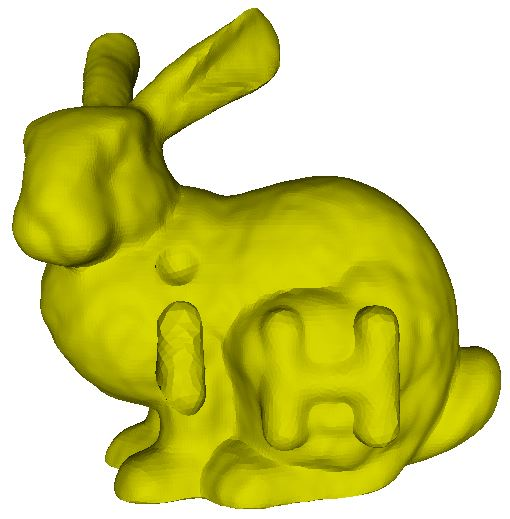
\includegraphics[width = 1.8cm]{results/bunny_PG15.jpg}}
\subfigure
{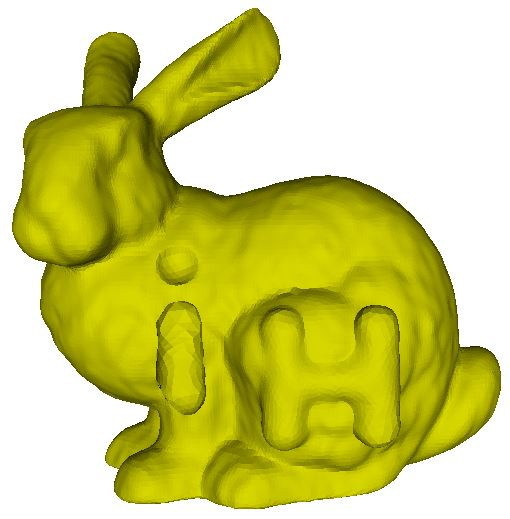
\includegraphics[width = 1.8cm]{results/bunny_our.jpg}}
\\
\vspace{-1.2mm}

\subfigure
{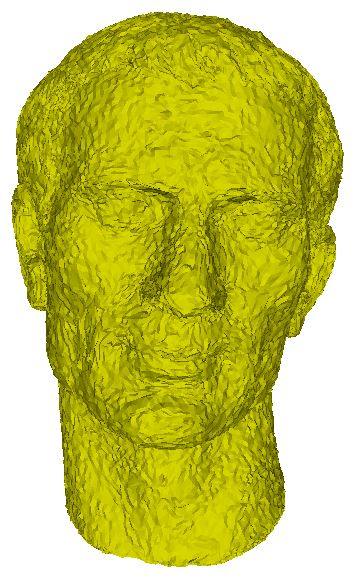
\includegraphics[width = 1.8cm]{results/julius_Noisy.jpg}}
\subfigure
{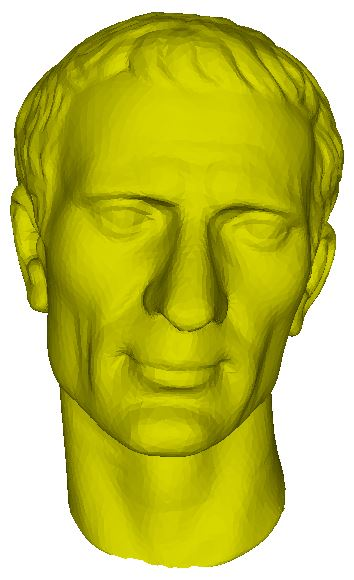
\includegraphics[width = 1.8cm]{results/julius_Original.jpg}}
\subfigure
{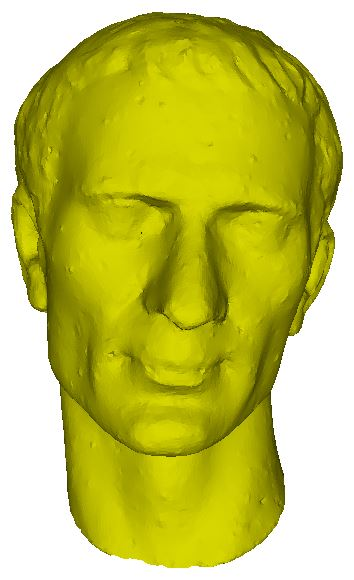
\includegraphics[width = 1.8cm]{results/julius_FDCO03.jpg}}
\subfigure
{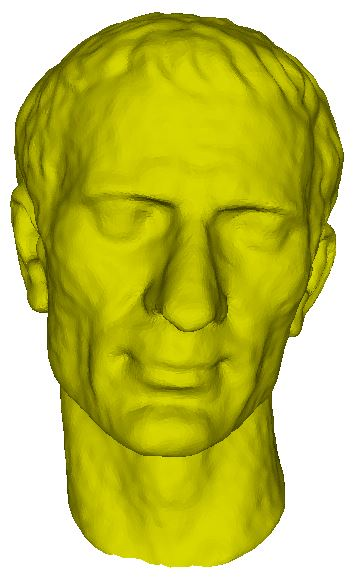
\includegraphics[width = 1.8cm]{results/julius_JDD03.jpg}}
\subfigure
{\includegraphics[width = 1.8cm]{results/julius_SRML07.jpg}}
\subfigure
{\includegraphics[width = 1.8cm]{results/julius_ZFAT11local.jpg}}
\subfigure
{\includegraphics[width = 1.8cm]{results/julius_HS13.jpg}}
\subfigure
{\includegraphics[width = 1.8cm]{results/julius_PG15.jpg}}
\subfigure
{\includegraphics[width = 1.8cm]{results/julius_our.jpg}}
\caption{ Comparisons with other methods on synthetic meshes. The results are from left to right noisy mesh, original mesh
, Fleishman et al~\cite{fleishman2003bilateral}, Jones et al~\cite{jones2003non}, Sun et al~\cite{sun2007fast},
Zheng et al~\cite{zheng2011bilateral}(l), He et al~\cite{he2013mesh}, Zhang et al~\cite{Zhang2015Filter} and our result separately. }
\label{Fig:datasets}
\end{figure*}

\begin{figure*}[htb]
\centering
\includegraphics[width = 15.0cm]{results/truemesh.jpg}
\vspace{0.5mm}
\caption{ true mesh.}
\label{Fig:relation}
\end{figure*}

\begin{table*}[ht]
\caption{Quantitative comparisons using two error metrics.}
\label{tab:1}
\begin{center}
\begin{tabular}{|c|c|c|c|c|c|c|c|c|} %% this creates eight columns also can be "c" and "r", "|" representative inserting ����
%% |l|l| to left justify each column entry
%% |c|c| to center each column entry
%% use of \rule[]{}{} below opens up each row
\hline
\rule[-1ex]{0pt}{3.5ex}  Model & Error  &  Fleishman~\cite{fleishman2003bilateral}  & Jones~\cite{jones2003non} & Sun~\cite{sun2007fast} & Zheng~\cite{zheng2011bilateral}(l) & He~\cite{he2013mesh} & Zhang~\cite{Zhang2015Filter} & ours \\
\hline\hline

\rule[-1ex]{0pt}{3.5ex}  \multirow{2}{*}{Fandisk}
& $N_{mean}$ & 9.7324 & 9.8179 & 4.0427 & 3.3494 & 5.5285 & 2.6239 & \textbf{2.3635} \\
\cline{2-9}
& $V_{mean}$ & 0.0181 & 0.0151 & 0.0110 & 0.0087 & 0.0188 & \textbf{0.0063} & 0.0065\\
\hline

\rule[-1ex]{0pt}{3.5ex}  \multirow{2}{*}{octahedron}
& $N_{mean}$ & 12.8072 & 10.6538 & 6.8467 & 5.2700 & 3.3284 & 3.3646 & \textbf{1.3607} \\
\cline{2-9}
& $V_{mean}$ & 0.0280 & 0.0147 & 0.0107 & 0.0063 & 0.0108 & 0.0049 & \textbf{0.0033}\\
\hline

\rule[-1ex]{0pt}{3.5ex}  \multirow{2}{*}{sphere}
& $N_{mean}$ & 12.5796 & 17.3618 & 11.8920 & \textbf{6.7047} & 12.9566 & 10.1697 & 7.2186 \\
\cline{2-9}
& $V_{mean}$ & 0.1551 & 0.0846 & 0.0888 & 0.0448 & 0.1241 & 0.0565 & \textbf{0.0446}\\
\hline

\rule[-1ex]{0pt}{3.5ex}  \multirow{2}{*}{bunny}
& $N_{mean}$ & 6.9293 & 5.8121 & 5.8896 & 5.6752 & 7.2142 & 5.3541 & \textbf{5.2400} \\
\cline{2-9}
& $V_{mean}$ & 0.0018 & 0.0009 & 0.0010 & 0.0009 & 0.0011 & 0.0008 & \textbf{0.0007}\\
\hline

\rule[-1ex]{0pt}{3.5ex}  \multirow{2}{*}{Julius}
& $N_{mean}$ & 7.7019 & 7.6301 & 7.0102 & 6.2115 & 7.9774 & 6.3760 & \textbf{6.1030} \\
\cline{2-9}
& $V_{mean}$ & 0.0011 & 0.0008 & \textbf{0.0006} & \textbf{0.0006} & 0.0009 & \textbf{0.0006} & \textbf{0.0006}\\
\hline

\rule[-1ex]{0pt}{3.5ex}  \multirow{2}{*}{block}
& $N_{mean}$ & 12.7155 & 13.8501 & 5.8023 & 5.3062 & 4.9734 & 3.5720 & \textbf{3.1134} \\
\cline{2-9}
& $V_{mean}$ & 0.1798 & 0.1335 & 0.0821 & 0.0680 & 0.1160 & 0.0541 & \textbf{0.0511}\\
\hline

\rule[-1ex]{0pt}{3.5ex}  \multirow{2}{*}{Nicolo}
& $N_{mean}$ & 8.8758 & 7.1305 & 6.3777 & \textbf{5.7978} & 7.5825 & 6.5012 & 5.9324 \\
\cline{2-9}
& $V_{mean}$ & 0.4604 & 0.3333 & 0.3184 & 0.2590  & 0.3475 & 0.2605 & \textbf{0.2499}\\
\hline

\rule[-1ex]{0pt}{3.5ex}  \multirow{2}{*}{twelve}
& $N_{mean}$ & 11.7204 & 11.0930 & 7.4519 & 7.3683 & 8.4624 & 2.7542 & \textbf{1.8934} \\
\cline{2-9}
& $V_{mean}$ & 0.0208 & 0.0173 & 0.0121 & 0.0125  & 0.0201 & 0.0.0062 & \textbf{0.0054}\\
\hline

\end{tabular}
\end{center}
\end{table*}

